\documentclass[a4paper]{article}

%%%%%%%% CREATE DOCUMENT STRUCTURE %%%%%%%%
%% Language and font encodings
\usepackage[english]{babel}
\usepackage[utf8x]{inputenc}
\usepackage[T1]{fontenc}
%\usepackage{subfig}

%% Sets page size and margins
\usepackage[a4paper,top=3cm,bottom=2cm,left=2cm,right=2cm,marginparwidth=1.75cm]{geometry}

%% Useful packages
\usepackage{amsmath}
\usepackage{amssymb}
\usepackage{graphicx}
\usepackage[toc,page]{appendix}
\setlength{\marginparwidth }{2cm}
\usepackage[colorinlistoftodos]{todonotes}
\usepackage[colorlinks=true, allcolors=blue]{hyperref}
\usepackage{caption}
\usepackage{subcaption}
\usepackage{sectsty}
\usepackage{apacite}
\usepackage{float}
\usepackage{titling} 
\usepackage{blindtext}
\usepackage[square,sort,comma,numbers]{natbib}
\usepackage{xcolor}
\usepackage{mathtools}
\usepackage{bbold}
\usepackage{tikz}
\usetikzlibrary{arrows,automata,positioning}
\usepackage{dsfont}
\usepackage{listings}
\usepackage{color} %red, green, blue, yellow, cyan, magenta, black, white
\definecolor{mygreen}{RGB}{28,172,0} % color values Red, Green, Blue
\definecolor{mylilas}{RGB}{170,55,241}

\newcommand{\R}{\mathbb{R}}
\definecolor{darkgreen}{rgb}{0.0, 0.4, 0.0}

%%%%%%%% DOCUMENT %%%%%%%%
\begin{document}
\lstset{language=Matlab,%
    %basicstyle=\color{red},
    breaklines=true,%
    morekeywords={matlab2tikz},
    keywordstyle=\color{blue},%
    morekeywords=[2]{1}, keywordstyle=[2]{\color{black}},
    identifierstyle=\color{black},%
    stringstyle=\color{mylilas},
    commentstyle=\color{mygreen},%
    showstringspaces=false,%without this there will be a symbol in the places where there is a space
    numbers=left,%
    numberstyle={\tiny \color{black}},% size of the numbers
    numbersep=9pt, % this defines how far the numbers are from the text
    emph=[1]{for,end,break},emphstyle=[1]\color{red}, %some words to emphasise
    %emph=[2]{word1,word2}, emphstyle=[2]{style},    
}
%%%% Title Page
\begin{titlepage}

\newcommand{\HRule}{\rule{\linewidth}{0.5mm}} 							% horizontal line and its thickness
\center 
 
% University
\textsc{\LARGE Delft University of Technology}\\[1cm]

% Document info
\textsc{\Large Modeling and Control of Hybrid Systems}\\[0.2cm]
\textsc{\large (SC42075)}\\[1cm] 										% Course Code
\HRule \\[0.8cm]
{ \huge \bfseries Assignment 2020}\\[0.7cm]								% Assignment
\HRule \\[2cm]
\large
\emph{Authors:}\\
Thijs Veen (4580060)\\
Maarten ten Voorde (4590740)\\[1.5cm]													% Author info
{\large \today}\\[5cm]

\includegraphics[width=0.6\textwidth]{images/TU_delft_logo.jpg}\\[1cm] 	% University logo
\vfill 
\end{titlepage}

% \begin{abstract}

% \end{abstract}

%%%% SECTIONS
\section{Part 1: Hybrid system example}
In Step 1.1 a description of a adaptive cruise control (ACC) system will be given and in Step 1.2 the system will be described as a hybrid automaton. 

\subsection*{Step 1.1}
Adaptive cruise control (ACC) is a more advanced version of the standard cruise control. ACC is able to control the car's speed and following distance to the car in front without communicating between the each other while the standard cruise control only controlled the speed without taking into account the distance to the car in front. The controller aims to keep the speed of the car equal to the set reference speed but may choose to slow down when the distance to the next car is lower than the set reference distance, this happens when the car in front suddenly brakes or when a car shifts into your lane.
Every car manufacturer implements different features into their ACC but some of the basic% features are:
\begin{itemize}
    % \item If the set speed button is pressed the ACC turns on with the current speed as the reference speed
    % \item If the distance to the next car is lower then a certain reference, slow down
    % \item If the current speed is slower then the reference speed and the distance to the next car is greater then the reference distance, try to accelerate back to the reference speed.
    % \item If the driver brakes or pushes the off button, turn of the ACC.
    
    \item If the set speed button is pressed the ACC turns on with the current speed as the reference speed
    \item If the distance to the next car is lower then a certain reference, slow down
    \item If the current speed is slower then the reference speed and the distance to the next car is greater then the reference distance, try to accelerate back to the reference speed.
    \item If the driver brakes or pushes the off button, turn of the ACC.
\end{itemize}

\subsection*{Step 1.2}

\section{Part 2: Energy management of microgrids}
subsection*{Step 2.1}
\begin{table}[]
\centering
\begin{tabular}{clclclc}
Variables related to the battery &  & Name &  & Range &  & Unit \\ \cline{1-1} \cline{3-3} \cline{5-5} \cline{7-7} 
Stored energy &  & $x_b$ &  & $[0,\bar{x}_b]$ &  & kWh \\
Exchanged power &  & $u_b$ &  & $[\underbar{$u$}_b,\bar{u}_b]$ &  & kW \\
Operational mode (charge/discharge) &  & $s_b$ &  & \{0,1\} &  & - \\
Charging efficiency &  & $\eta_c$ &  & CONSTANT &  & - \\
Discharging efficiency &  & $\eta_d$ &  & CONSTANT &  & -
\end{tabular}
\caption{Parameters related to the battery}
\label{batteryParm}
\end{table}

The battery can be modelled as a discrete-time piecewise affine (PWA) system with the state being the energy stored in the battery and the input being the exchanged power from the perspective of the grid, which means that it has a negative sign when the battery is being charged and a positive sign when the battery is discharging energy to the grid. The model can then be constructed as follows
\begin{equation*}
f(x_b(k),u_b(k)) =\left\{\begin{matrix}
x_b(k)-\eta_c T_s u_b(k), & \text{if } u_b(k) \leq 0 \\
x_b(k)-\eta_d T_s u_b(k), & \text{if } u_b(k) > 0 
\end{matrix}\right.
\end{equation*}
where $x_b(k) \in [0,\bar{x}_b]$ and $u_b(k) \in [\underbar{$u$}_b, \bar{u}_b]$.

\subsection*{Step 2.2}
After introducing the following constraints, the PWA system can be cast into a MLD system
$$
\begin{array}{l}
0 \leq x_{\mathrm{b}}(k) \leq \bar{x}_{\mathrm{b}} \\
\underline{u}_{\mathrm{b}} \leq u_{\mathrm{b}}(k) \leq \bar{u}_{\mathrm{b}} \\
\text { if } s_{\mathrm{b}}(k)=1 \Rightarrow u_{\mathrm{b}}(k) \leq 0 \\
\text { if } s_{\mathrm{b}}(k)=0 \Rightarrow u_{\mathrm{b}}(k)>0
\end{array}
$$
The general MLD form is as follows
$$
\begin{array}{l}
x(k+1)=A x(k)+B_{1} u(k)+B_{2} \delta(k)+B_{3} z(k)+B_{4} \\
E_{1} x(k)+E_{2} u(k)+E_{3} \delta(k)+E_{4} z(k) \leq g_{5}
\end{array}
$$
To determine the matrices $A$, $B_i$, $E_i$ and $g_5$, the binary variable $\delta(k)$ is introduced to the condition $s_b(k) = 1$
$$
[\delta(k) = s_b(k) = 1] \Leftrightarrow [u_b(k) \leq 0]
$$
This condition is true iff
\begin{align*}
u_b(k) &\leq \bar{u}_b(1-\delta(k))\\
u_b(k) &\geq \epsilon + (\underline{u}_b-\epsilon)\delta(k))
\end{align*}
The bounds on the state $u_b$ can be expressed as, with auxiliary $z(k) = \delta(k)z(k)$
$$
\begin{array}{l}
z(k) \leq \bar{u}_b \delta(k) \\
z(k) \geq \underline{u}_b \delta(k) \\
z(k) \leq u_b(k)-\underline{u}_b(1-\delta(k)) \\
z(k) \geq u_b(k)-\bar{u}_b(1-\delta(k))
\end{array}
$$
Since the bounds on $x_b$ do not depend on decision variable $s_b(k)$, they can be directly incorporated to the general MLD form. There are six constraints on the input, and two constraints on the state, so the general MLD form becomes
\begin{align}
    f(x_b(k),u_b(k)) &= x_b(k) - (\eta_c - \eta_d)T_s\delta(k)u_b(k) - \eta_dT_su_b(k) \nonumber\\
    f(x_b(k),u_b(k)) &= x_b(k) - (\eta_c - \eta_d)T_sz(k) - \eta_dT_su_b(k) \label{eq:2.1MLDdynamics}
\end{align}
with the constraints
From equation \ref{eq:2.1MLDdynamics} it follows that $A = 1$, $B_1 = \eta_dT_s$, $B_2 = 0$, $B_3 = (\eta_c - \eta_d)T_s$ and $B_4 = 0$. $E_1,\dots,E_4,g_5$ are vectors that contain the MLD system inequality values, which are equal to
$$
\underbrace{\begin{bmatrix} -1 \\ 1 \\ 0 \\ 0 \\ 0 \\ 0 \\ 0 \\ 0 \\ 0 \\ 0 \end{bmatrix}}_{E_1}x_b(k) + 
\underbrace{\begin{bmatrix} 0 \\ 0 \\ -1 \\ 1 \\ 1 \\ -1 \\ 0 \\ 0 \\ -1 \\ 1 \end{bmatrix}}_{E_2}u_b(k) + 
\underbrace{\begin{bmatrix} 0 \\ 0 \\ 0 \\ 0 \\ -\bar{u}_b \\ (\underline{u}_b-\epsilon) \\ -\bar{u}_b \\ \underline{u}_b \\ -\underline{u}_b \\ \bar{u}_b \end{bmatrix}}_{E_3}\delta(k) +
\underbrace{\begin{bmatrix} 0 \\ 0 \\ 0 \\ 0 \\ 0 \\ 0 \\ 1 \\ -1 \\ 1 \\ -1 \end{bmatrix}}_{E_4}z(k) \leq
\underbrace{\begin{bmatrix} 0 \\ \bar{x}_b \\ -\underline{u}_b \\ \bar{u}_b \\ \bar{u}_b \\ -\epsilon \\ 0 \\ 0 \\ -\underline{u}_b \\ \bar{u}_b \end{bmatrix}}_{g_5}
$$
\subsection*{Step 2.3}
\label{sec:2.3}
To determine the values of $a_i$ and $b_i$ for $i \in \{1,2,3,4\}$ that minimizes the squared area between $f$ and $\hat{f}$, 
\begin{align}
    \int_{0}^{\bar{u}_{d}}\left(f\left(u_{\mathrm{d}}\right)-\hat{f}\left(u_{\mathrm{d}}\right)\right)^{2} d u_{\mathrm{d}} \label{eq:2.3cost}
\end{align}
a new PWA function of $f(u_d)-\hat{f}(u_d)$ has been created where the regions of $f(u_d)$ have been synced with the four functions of $\hat{f}(u_d)$. This created four separate minimization problems which have been minimized with \textit{fmincon()}. Equailty constraints were used, so that the functions have the same function value at the boundary. The steps to arrive at the given solutions are:
\begin{enumerate}
    \item Approximate the first part, results in $a_1$ and $b_1$.
    \item Compute $\hat{f}(u_d)$ at the end of the first part (at $u_d$ = 5).
    \item Solve for the second part $(5\leq u_d<6.5)$ with an equality constraint $a_1+5b_1 = a_2+5b_2$.
    \item Repeat this for all parts, with the appropriate bounds and parameters
\end{enumerate}
The optimal variables are shown in table \ref{tab:2.3table}, and figure \ref{fig:part23} shows $\hat{f}(u_d)$.\\
\begin{table}[h]
    \centering
    \caption{The optimal variables $a_i$, $b_i$}
    \begin{tabular}{c|c|c|c}
    \hline
         $a_1$ &  1.8133 & $b_1$ & 3.488 \\
         $a_2$ &  -83.647 & $b_2$ & 20.58  \\
         $a_3$ &  110.08 & $b_3$ & -9.2246 \\
         $a_4$ &  -212.98 & $b_4$ & 20.144   
    \end{tabular}
    
    \label{tab:2.3table}
    \end{table}
A Matlab script \ref{} has been created to perform this PWA approximation, which can be examined for further explanation.
\begin{figure}[ht]
    \centering
    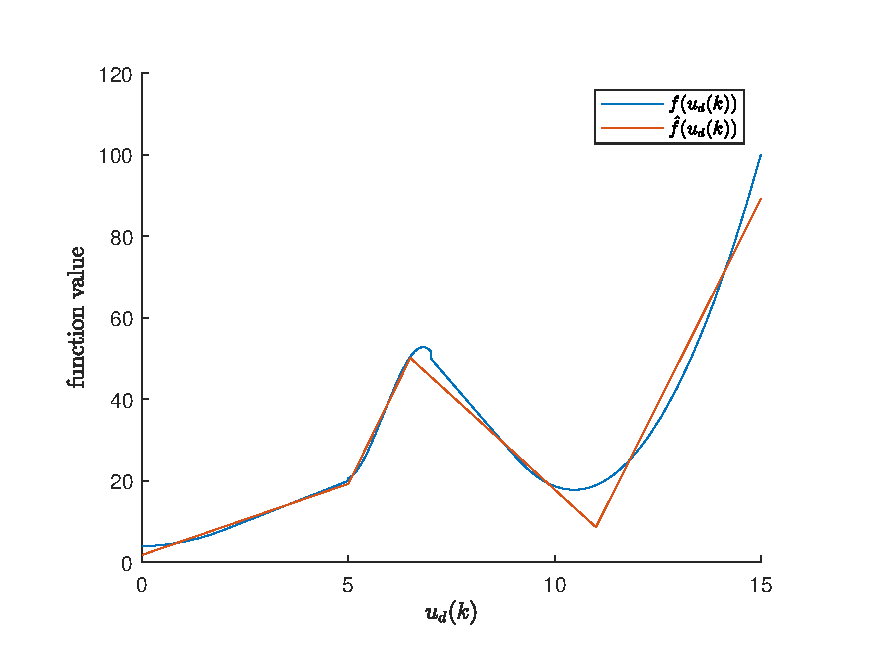
\includegraphics[width=0.8\textwidth]{Latex/images/step23.pdf}
    \caption{PWA approximation comparison}
    \label{fig:part23}
\end{figure}

\subsection*{Step 2.4}
The aim is to determine the values of $a_i$ and $b_i$ for $i \in \{1,2,3,4\}$, and $u_j$  for $j \in \{1,2,3\}$, that minimizes cost function \ref{eq:2.3cost}. Similarly to section \ref{sec:2.3}, \textit{fmincon()} is used, but the steps to compute the minimum are different. The method to compute $a_i$, $b_i$ and $j_i$ is
\begin{enumerate}
    \item Create a function that contains
    \begin{itemize}
        \item A symbolic piecewise function $f(u_d)$.
        \item A symbolic piecewise function $\hat{f}(u_d,a_i,b_i,u_i)$.
        \item The cost \ref{eq:2.3cost}, using the symbolic piecewise functions.
    \end{itemize}
    \item Create the nonlinear constraints that represent the boundary conditions
    \item Use \textit{fmincon()} to minimize the function, with the nonlinear constraints
\end{enumerate}
The nonlinear constraints are 
\begin{align*}
    a_1 + b_1u_1 - (a_2+b_2u_1) = 0\\
    a_2 + b_2u_2 - (a_3+b_3u_2) = 0\\
    a_3 + b_3u_3 - (a_4+b_4u_3) = 0
\end{align*}
The result is shown in figure \ref{fig:part24}. The computed optimal parameters are (table \ref{tab:2.4table}
\begin{table}[h]
    \centering
    \caption{The optimal variables $a_i$, $b_i$ and $j_i$}
    \begin{tabular}{c|c|c|c|c|c}
    \hline
         $a_1$ &  1.7417 & $b_1$ & 3.5305 & $u_1$ & 5.1192\\
         $a_2$ &  -96.394 & $b_2$ & 22.701 & $u_2$ & 6.5093\\
         $a_3$ &  107.42 & $b_3$ & -8.6111 & $u_3$ & 11.236\\
         $a_4$ &  -227.93 & $b_4$ & 21.236 &  &  
    \end{tabular}
    \label{tab:2.4table}
\end{table}
The Matlab file can be found in \ref{}
\begin{figure}
    \centering
    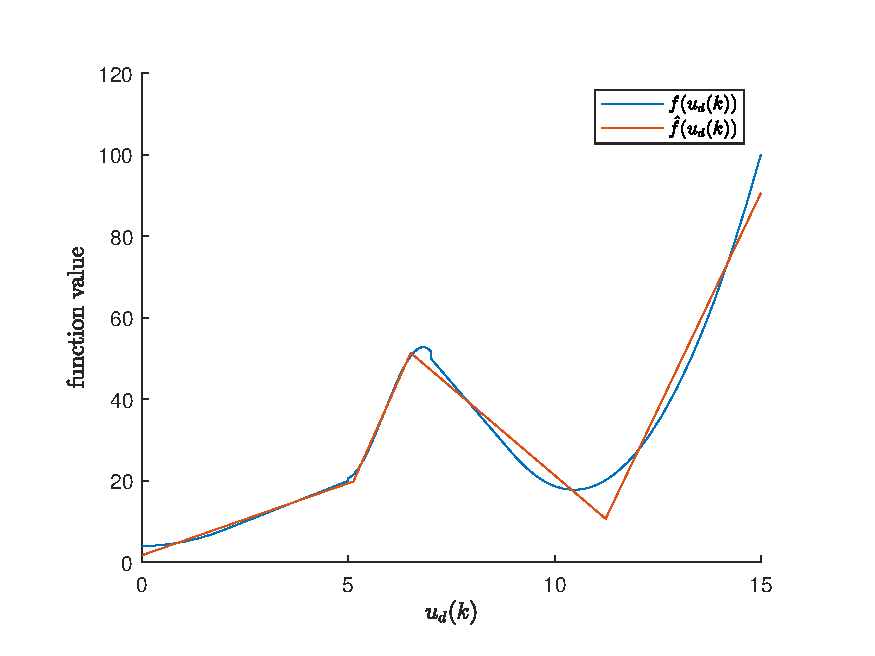
\includegraphics[width=0.8\textwidth]{Latex/images/step24.pdf}
    \caption{PWA approximation comparison, with optimized $u_i$}
    \label{fig:part24}
\end{figure}
\subsection*{Step 2.5}
A discrete-time PWA model of the diesel generator's fuel tank can be constructed, where the state is the fuel level in the tank and the input is the generated power. The fuel tank is constantly being refuelled with a constant rate of $R_f$ kg/h and a switching signal $s_d$ that indicates the on/off operational mode of the generator. The model can then be constructed as follows
\begin{equation}
f(x_d(k),u_d(k)) = x_d(k) + T_sR_f - s_d(k)\hat{f}(u_d(k)) \label{eq:PWA25}
\end{equation}
with $T_s$ a time step and
$$
\hat{f}\left(u_{\mathrm{d}}(k)\right)=\left\{\begin{array}{ll}
a_{1}+b_{1} u_{\mathrm{d}}(k) & \text { if } 0 \leq u_{\mathrm{d}}(k)<u_{1} \\
a_{2}+b_{2} u_{\mathrm{d}}(k) & \text { if } u_{1} \leq u_{\mathrm{d}}(k)<u_{2} \\
a_{3}+b_{3} u_{\mathrm{d}}(k) & \text { if } u_{2} \leq u_{\mathrm{d}}(k)<u_{3} \\
a_{4}+b_{4} u_{\mathrm{d}}(k) & \text { if } u_{3} \leq u_{\mathrm{d}}(k) \leq 15
\end{array}\right.
$$
where the values of $a_i$ and $b_i$ for $i \in \{1,2,3,4\}$ are given in table \ref{tab:2.4table} and the values of $u_1$, $u_2$ and $u_3$ are given in the problem description of Step 2.3.
\subsection*{Step 2.6}

\begin{align*}
& \underline{x}_D \leq x_d(k) \leq \Bar{x}_d \\
& 0 \leq u_d(k) \leq \Bar{u}_d \\
& \text{if } s_d(k) = 0 \Rightarrow \text{there is no power generation at time step } k 
\end{align*}

\begin{align*}
[\delta_1 = 1] \Leftrightarrow [u_d(k) \geq 0] \text{ true iff}
&\left\{\begin{matrix*}[l]
    -u_d(k) \leq 0 \\
    u_d(k) - (u_1 + \epsilon)\delta_i(k) \leq -\epsilon
\end{matrix*}\right. \\
[\delta_2 = 1] \Leftrightarrow [u_d(k)-u_1 \geq 0] \text{ true iff}
&\left\{\begin{matrix*}[l]
    -u_d(k) -u_1\delta_2(k) \leq -2u_1 \\
    u_d(k) - (u_2 + \epsilon)\delta_i(k) \leq -\epsilon + u_1
\end{matrix*}\right. \\
[\delta_3 = 1] \Leftrightarrow [u_d(k)-u_2 \geq 0] \text{ true iff}
&\left\{\begin{matrix*}[l]
    -u_d(k) -u_2\delta_3(k) \leq -2u_2 \\
    u_d(k) - (u_3 + \epsilon)\delta_i(k) \leq -\epsilon + u_2
\end{matrix*}\right. \\
[\delta_4 = 1] \Leftrightarrow [u_d(k)-u_3 \geq 0] \text{ true iff}
&\left\{\begin{matrix*}[l]
    -u_d(k) -u_3\delta_4(k) \leq -2u_3 \\
    u_d(k) - (\Bar{u}_d + \epsilon)\delta_i(k) \leq -\epsilon + u_3
\end{matrix*}\right.
\end{align*}

$$
\hat{f}(u_d(k)) = \delta_1(a_1+b1u_d(k)) + \delta_2(a_2+b2u_d(k)) + \delta_3(a_3+b3u_d(k)) + \delta_4(a_4+b4u_d(k)) 
$$

% $$
% [\delta_2 = 1] \Leftrightarrow [u_1-u_d(k) \leq 0] \text{ true iff }
% \left\{\begin{matrix*}[l] -u_d(k) \leq u_2(1-\delta_2)-u_1 \\ u_d(k) \geq \epsilon + (m-\epsilon)\delta_2 \ \end{matrix*}\right.
% $$

% $$
% [\delta_2 = 1] \Leftrightarrow [u_1-u_d(k) \leq 0] \text{ true iff }
% \left\{\begin{matrix*}[l] \\ \end{matrix*}\right.
% $$

% the Mixed logical dynamical (MLD) system can then be constructed as  
\subsection*{Step 2.7}
A system with several parts can be stacked. The matrices corresponding to the diesel model and batteries are represented as $A_{d}$, $B_{i_{d}}$ $E_{i_{d}}$, $g_{i_{d}}$, and $A_{bj}$, $B_{i_{bj}}$ $E_{i_{bj}}$, $g_{i_{bj}}$ respectively. $_{bj}$ corresponds to the $j^{th}$ battery. The dynamics of a diesel generator and two batteries become
\begin{align*}
    \begin{bmatrix} x_d(k+1)\\ x_{b1}(k+1)\\x_{b1}(k+1)\end{bmatrix} &= \begin{bmatrix} A_d & 0 & 0\\ 0 & A_{b1} & 0\\ 0 & 0 & A_{b2}\end{bmatrix}\begin{bmatrix} x_d(k)\\ x_{b1}(k)\\x_{b2}(k)\end{bmatrix}
    + \begin{bmatrix} B_{1_{d}} & 0 & 0\\ 0 & B_{1_{b1}} & 0\\ 0 & 0 & B_{1_{b2}}\end{bmatrix}\begin{bmatrix} u_d(k)\\ u_{b1}(k)\\u_{b2}(k)\end{bmatrix} \\
    &+ \begin{bmatrix} B_{2_{d}} & 0 & 0\\ 0 & B_{2_{b1}} & 0\\ 0 & 0 & B_{2_{b2}}\end{bmatrix}\begin{bmatrix} \delta_d(k)\\ \delta_{b1}(k)\\\delta_{b2}(k)\end{bmatrix}
    + \begin{bmatrix} B_{3_{d}} & 0 & 0\\ 0 & B_{3_{b1}} & 0\\ 0 & 0 & B_{3_{b2}}\end{bmatrix}\begin{bmatrix} z_d(k)\\ z_{b1}(k)\\z_{b2}(k)\end{bmatrix} 
    + \begin{bmatrix} B_{5_{d}}\\ B_{5_{b1}}\\B_{5_{b2}}\end{bmatrix}
\end{align*}
Similarly for the constraints
\begin{align*}
    &\begin{bmatrix} E_{1_{d}} & 0 & 0\\ 0 & E_{1_{b1}} & 0\\ 0 & 0 & E_{1_{b2}}\end{bmatrix}
    \begin{bmatrix} x_d(k)\\ x_{b1}(k)\\x_{b2}(k)\end{bmatrix}
    + \begin{bmatrix} E_{2_{d}} & 0 & 0\\ 0 & E_{2_{b1}} & 0\\ 0 & 0 & E_{2_{b2}}\end{bmatrix}\begin{bmatrix} u_d(k)\\ u_{b1}(k)\\u_{b2}(k)\end{bmatrix} \\
    + &\begin{bmatrix} E_{3_{d}} & 0 & 0\\ 0 & E_{3_{b1}} & 0\\ 0 & 0 & E_{3_{b2}}\end{bmatrix}\begin{bmatrix} \delta_d(k)\\ \delta_{b1}(k)\\\delta_{b2}(k)\end{bmatrix}
    + \begin{bmatrix} E_{4_{d}} & 0 & 0\\ 0 & E_{4_{b1}} & 0\\ 0 & 0 & E_{4_{b2}}\end{bmatrix}\begin{bmatrix} z_d(k)\\ z_{b1}(k)\\z_{b2}(k)\end{bmatrix} 
    \leq \begin{bmatrix} g_{5_{d}}\\ g_{5_{b1}}\\g_{5_{b2}}\end{bmatrix}
\end{align*}
These equations can be rewritten in vector-matrix form
\setcounter{MaxMatrixCols}{20}
\begin{align}
    \underbrace{\begin{bmatrix} x(k+1)\\ x(k+2)\\\vdots\\x(k+l)\end{bmatrix}}_{\tilde{x}(k)} &=  \underbrace{\begin{bmatrix*}
    B_1 & 0 & \dots & 0 &                   B_2 & 0 & \dots & 0 &                   B_3  & 0 & \dots & 0\\
    AB_1& B_1 &  & \vdots &                 AB_2& B_2 &  & \vdots &                 AB_3 & B_3 &  & \vdots\\
    \vdots&  & \ddots & 0 &                 \vdots&  & \ddots & 0 &                 \vdots &  & \ddots & 0\\
    A^{l}B_1&  A^{l-1}B_1 & \dots &  B_1 & A^{l}B_2 &  A^{l-1}B_2 & \dots &  B_2 & A^{l}B_3 &  A^{l-1}B_3 & \dots &  B_3\end{bmatrix*}}_{M_1}\tilde{V}(k)\nonumber\\
    &+ \underbrace{\begin{bmatrix} A\\A^2\\\vdots\\A^{l+1}\end{bmatrix}}_{M_2}x(k) +  \underbrace{\begin{bmatrix} I_3\\A+I_3\\\vdots\\A^{l} + A^{l-1} \dots + 1 \end{bmatrix}}_{M_3}B_4 \label{eq:step27_tildedyn}
\end{align}
where $\tilde{V}(k)$ denotes all the unknowns
$$
    \tilde{V}(k)  =\begin{bmatrix} u(k)& \dots& u(k+l)& \delta(k)& \dots& \delta(k+l)& z(k) & \dots & z(k+l)\end{bmatrix}^T
$$
The constraints become 
\setcounter{MaxMatrixCols}{12}
\begin{gather}
    \underbrace{\begin{bmatrix} E_1A^{l-1}B_1 &\dots& E_1B1 & E_2 & E_1A^{l-1}B_2 & \dots & E_1B_2 & E_3 & E_1A^{l-1}B_3 & \dots & E_1B_3 & E_4 \end{bmatrix}}_{F_1} \tilde{V}(k)\nonumber\\
    + \underbrace{E_1A^l}_{F_3}x(k)\leq g_5 \label{$eq:step27_F$}
\end{gather}
This matrix-vector notation allows for optimisation algorithms, since these algorithms often use the form $Fx\leq b$ .
\subsection*{Step 2.8}
The cost function $J(k)$ 
\begin{align*}
    J(k) &= \sum^{N_p-1}_{j=0} ( \sum^{N_b-}_{i=1}W_{b,i}|\Delta s_{b,i}(k+j)| + W_d|\Delta s_{d}(k+j)|\\
    &- W_{\text{fuel}}(x_d(l+N_p) - x_d(k) - W_e\sum^{N_b-}_{i=1}(x_{b,i}(k+N_p) - x_{b,i}(k))\\
    &+ \sum^{N_p-1}_{j=0} P_{\text{imp}}(k+j)C_e(k+j)
\end{align*}
contains $|\Delta s_{b,i}(k+j)|$ and $W_d|\Delta s_{d}(k+j)|$. The absolute value is not a linear term, so the optimisation problem is not a linear programming problem. The problem can be recast into a linear programming problem by introducing a dummy variable $p$ and some constraints on the dummy variable. The first line of the cost function becomes
\begin{align*}
   \min_{p_i} &\sum^{N_p-1}_{j=0} (W_dp_1(k+j) + W_{b,1}p_2(k+j) + W_{b,2}p_3(k+j))\\
   \text{s.t.} \indent& -p_1(k+j) - s_d(k+j) + s_d(k+j-1) \leq 0 \indent \forall j > 0\\
   & -p_1(k+j) + s_d(k+j) - s_d(k+j-1) \leq 0 \indent \forall j > 0\\
   & -p_{2}(k+j) - s_{b,1}(k+j) + s_{b,1}(k+j-1) \leq 0 \indent \forall j > 0\\
   & -p_{2}(k+j) + s_{b,1}(k+j) - s_{b,1}(k+j-1) \leq 0 \indent \forall j > 0\\
   & -p_{3}(k+j) - s_{b,2}(k+j) + s_{b,2}(k+j-1) \leq 0 \indent \forall j > 0\\
   & -p_{3}(k+j) + s_{b,2}(k+j) - s_{b,2}(k+j-1) \leq 0 \indent \forall j > 0\\
   & -p_1(k+j) - s_d(k+j)  \leq - s_d(-1) \indent \forall j = 0\\
   & -p_1(k+j) + s_d(k+j)  \leq s_d(-1) \indent \forall j = 0\\
   & -p_2(k+j) - s_{b,1}(k+j)  \leq - s_{b,1}(-1) \indent \forall j = 0\\
   & -p_2(k+j) + s_{b,1}(k+j)  \leq s_{b,1}(-1) \indent \forall j = 0\\
   & -p_3(k+j) - s_{b,2}(k+j)  \leq - s_{b,2}(-1) \indent \forall j = 0\\
   & -p_3(k+j) + s_{b,2}(k+j)  \leq s_{b,2}(-1) \indent \forall j = 0\\
\end{align*}
An extra constraint is also added for $P_{imp}$
\begin{align}
P_{\text{imp}} + u_d(k+j) + u_{b,1}(k+j) + u_{b,2}(k+j) = P_{\text{load}} \indent f\forall j\label{eq:step28_eqcons}
\end{align}
Since $p$ and $P_{\text{imp}}$ are new optimisation variables, they are included in $\tilde{V}(k)$, so 
$$\tilde{V}(k) = \begin{bmatrix} \tilde{V}(k) \\ \tilde{p}_1(k) \\ \tilde{p}_2(k) \\ \tilde{p}_3(k)\\ \tilde{P}_{\text{imp}}(k) \end{bmatrix}$$
Matrices $M_i$ and $F_i$ will have to adjusted accordingly, which comes down to adding zeros to the right side of or beneath the matrices, since the qualities do not depend on dummy variable $\tilde{p}_i(k)$ and $\tilde{P}_{\text{imp}}$. The cost function can be, just as the qualities, written in vector matrix form. The aim is to write the cost function as a linear function of $\tilde{V}(k)$.
\begin{align*}
    J(k) &= \underbrace{\begin{bmatrix} 0 & \dots  & W_d\mathbb{1} & W_{b,1}\mathbb{1} & W_{b,2}\mathbb{1} & 0\end{bmatrix}}_{W_1} \tilde{V}(k)\\
    &+ \underbrace{\begin{bmatrix} W_{\text{fuel}} & W_e  & W_e & 0 & \dots &  -W_{\text{fuel}} & -W_e  & -W_e\end{bmatrix}}_{W_2} \tilde{x}(k) \\
    &+ \underbrace{\begin{bmatrix} 0 & \dots  & 0 & \tilde{C}_e(k)^T & W_{b,2}\mathbb{1} \end{bmatrix}}_{C_1}\tilde{V}(k)
\end{align*}
$\tilde{x(k)}$ can be substituted by \ref{eq:step27_tildedyn}, so that $J(k)$ becomes a function of only $\tilde{V}(k)$.
\begin{align*}
    J(k) &= W_1\tilde{V}(k) + W_2(M_1\tilde{V}(k)+M_2(x(k)+M_2) + C_1\tilde{V}(k) + \tilde{P}_{\text{load}}^T\tilde{C}_e\\
    &= (W_1 + W_2M_1 + C_1)\tilde{V}(k) + W_2M_2x(k) + W_2M_3 + \tilde{P}_{\text{load}}^T\tilde{C}_e
\end{align*}
Since the second part of the equation does not depend on $\tilde{V}(K)$, it does not influence the optimally, so the linear programming problem becomes
\begin{align*}
    \min_{\tilde{V}(k)} &(W_1 + W_2M_1 + C_1)\tilde{V}(k)\\
    \text{s.t} \indent &F_1\tilde{V}(k) \leq F_2 + F_3x(k)
\end{align*}
$F_2$ consists of the right hand side of the constraints, and $F_3$ is the $F_3$ matrix from equation \ref{$eq:step27_F$} but with added zeros, corresponding to variables $p_i$ and $P_{\text{imp}}$. Note that the constraints \ref{eq:step28_eqcons} is a equality constraint, so $\leq$ becomes $=$.


\subsection*{2.9}
We tried to solve the problem with gurobi, but the problem was unbounded. Adding upper bounds on the vector $\tilde{V}(k)$ made the solution feasible, until $P_{\text{load}}$ was not zero anymore. We suspect our error is in the constraints, but we do not know if it is in the derivation of the MLD model, or a coding error in the Matlab file. We have also tried to use YALMIP for the MPC, and it performed better, but it had very long computation time when $C_e$ neared zero, more than an hour for a single timestep. For YALMIP we did not vectorise the MLD model.
We have tried to find an error in our derivation and Matlab files, but we were unable to find one. Some things surprised us in our derivation, so it could be that the error lies there
\begin{itemize}
    \item The minimisation does not depend on the matrix $B_4$, since it disappears in our derivation because it does not depend on $\tilde{V}(k)$.
    \item When we tried to substitude the constraint for $P_{\text{imp}}$ into the cost function, the optimal $\tilde{V}(k)$ did not depend on $P_{\text{load}}$, so we added it as an constraint. With this constraint, $P_{\text{load}}$ influenced the feasibility.
\end{itemize}
\subsection*{Step 2.10}
Since our problem is infeasible, we cannot simulate. We can however express the constraints.
\begin{align*}
    -x_{b,i}(n\frac{12}{T_s}) \leq 0.2 \underline{x_{b,i}} \indent \forall i
\end{align*}
where $n$ is an integer
\newpage
\subsection*{Conclusion}
\subsubsection*{Part 1}
Adaptive cruise control is a system that is easily written as a hybrid automaton as it required only 3 modes and one discrete state to describe the dynamics of the system as described in Step 1.1. The size of the hybrid automaton of a ACC depends on the level of complexity of the ACC and as the ACC described in Step 1.1 was rather simple, the size of the hybrid automaton was kept to a minimum.   

% There are probably many different ways of creating a hybrid automaton of a Adaptive cruise control system,

% It could even be reduced to two nodes if the normal operation mode is left out and you start at $q_2$ and ...

\subsubsection*{Part 2}
Since we failed to simulate and compute the optimal control input, it is difficult to draw a conclusion about the performance of the MPC controller of this hybrid system. We have seen the potential of Model Predictive controllers in other situations, and we suspect that it is very much suited for hybrid systems, since MPC can deal with constraints, where most other control strategies cannot. Since the sampling time of this grid system is rather low, the MPC should not run into time issues due to computational complexity. Step 2.10 should show how very specific constraints, like a constraint on a single time step, can be incorporated into MPC. We cannot think of any other control method that allows for these kind of constraints/objectives.

\subsection*{Evaluation}
\subsubsection*{Part 1}
There are probably many different ways of creating a hybrid automaton of a Adaptive cruise control system, we managed to create one with 3 modes and one discrete state for turning the ACC on/off. This can probably be reduced even further by removing the normal operation mode ($q_1$) of the car and only describing the ACC part. But keeping mode $q_1$ creates a handy loop in which the system can switch between the driver taking control and the ACC controlling the car. The guard condition $G(q_1,q_2)$ depended on the distance between the two cars, which was not a state in the state description of mode $q_1$. This raised some questions whether it should be added to the state description of that mode or be viewed as a outside interrupt from the sensor. the latter has been chosen as the dynamics in that mode didn't depend on that state.\\
\\
Part 1 showed that any kind of dynamic can be modeled by a hybrid automaton, although the size and complexity can grow rapidly with more complex dynamics.

\subsubsection*{Part 2}
This assignment gave us the insight in how to model event-based models. Part 2 of the assignment learned us how to cast a, for us more intuitive, piecewise affine model into a MLD model. It became clear that the MLD model is very well suited for MPC. The recasting of model is a tedious task that requires accuracy and precision. Representing the MLD model in vector-matrix form was new for us. After vectoring the matrices, we noticed that there were more unknown variables than $u$, $\delta$ and $z$, so we had to alter the $M_i$ and $F_i$ matrices. If a similar problem arises now, we would first consider what all the unknown variables are, before we start vectorising.\\
\\
Furthermore, we were unable to find our mistake. We should have had more care in ensuring our answers were correct. After the simulation failed, it was too late to find the mistake. Since there was a large amount of constraints and unknowns, it is very difficult to inspect the matrices and see if they are correct.\\
\\
Additionally, it became apparent how easy it is to approximate a nonlinear function with a piecewise affine function. Connecting the boundaries was also trivial, since it came down to adding some equality constraints. The plots showed some good approximations, better than we expected.\\
\\
The most important thing learned for this assignment, is how many constraints there are for a relatively concise model of only three parts. A large part of the constraints are the result of the PWA function $\hat{f}$. Representing the MLD model with less decision and auxiliary variables would reduce the number of constraints, and thus the risk of a mistake. Taking the effort to use the most concise MLD model might take more time in creating the MLD model, but it is probably worth it, since it takes effort away later.\\
\\
Overall, this assignment is our first introduction with hybrid systems. It showed us available modeling structures, capable of capturing the switching dynamics. We understand the reason to write a model in MLD structure, since this structure can be recast into an optimisation problem. The PWA or hybrid automaton model could not directly be used for MPC. These types of assignments force you to delve deeper into the material than lectures and a written exam ever could.\\
\\
All the code can be found in \cite{GIT}, and in the appendices.


%%%%%%%% EXTRA TIPS %%%%%%%%
%% hou deze structuur aan voor afbeeldingen
%%\begin{figure}[H]
%%\includegraphics[]{Pendulum.jpg}
%%\caption{Sketch of the pendulum}
%%\label{fig:pendulum}
%%\end{figure}


%\newpage
\bibliographystyle{apacite}
\bibliography{ref.bib}
\newpage
\begin{appendices}
\lstinputlisting{step23.m}
\newpage
\lstinputlisting{step24.m}
\newpage
\lstinputlisting{step27.m}
\newpage
\lstinputlisting{step28fun.m}
\newpage
\lstinputlisting{step29.m}
\end{appendices}
\end{document}